\section{Correction} \label{Corr}
\graphicspath{{images/corr}}

\modif{Intro !}

\subsection{Presentation of different problems considered} \label{Corr.problems}

\modif{A faire au fur et à mesure !}

In this section, we present the different problems we'll be considering in Section \ref{Corr.results}. We will consider the geometry of a circle in Section \ref{Corr.pb.circle} represented in Figure \ref{geom_circle} as well as the geometry of a square in Section \ref{Corr.pb.square} represented in Figure \ref{geom_square}. We'll also look at different solutions \modif{à compléter (sol analytique-exacte vs sol de référence calculés avec FEM sur-raffinée)}.

\begin{minipage}{0.48\linewidth}
	\begin{figure}[H]
		\centering
		\includegraphics[width=0.6\linewidth]{"geom_circle.png"}
		\captionof{figure}{Representation of the first domain considered : the Circle.}
		\label{geom_circle}
	\end{figure} 
\end{minipage}
\begin{minipage}{0.48\linewidth}
	\begin{figure}[H]
		\centering
		\includegraphics[width=0.6\linewidth]{"geom_square.png"}
		\captionof{figure}{Representation of the second domain considered : the Square.}
		\label{geom_square}
	\end{figure} 
\end{minipage}

\begin{Rem}
	Note that in the case where the problem is non-homogeneous, we can consider
	\begin{equation*}
	g(x,y)=u_{ex}(x,y)\times(1+\phi(x,y))
	\end{equation*}
	with $\phi$ the levelset function, null by definition on $\Gamma$.
\end{Rem}

\subsubsection{First domain : the Circle.} \label{Corr.pb.circle}

Here, we'll consider the $\Omega$ domain to be the circle of radius $\sqrt{2}/4$ and center $(0.5,0.5)$.This domain is entirely included in the fictitious domain $O=[0,1]^2$ (Figure \ref{geom_circle}).

We will consider the levelset function $\phi$ defined by
\begin{equation*}
	\phi(x,y)=-1/8+(x-1/2)^2+(y-1/2)^2,
\end{equation*}
negative function inside the domain, null at the boundary and positive outside it
	
We then consider different problems \modif{à compléter}.

\paragraph{First problem} \label{Corr.pb.circle.1}

Here, we are interested in the Poisson problem with an analytical solution
\begin{equation*}
	u_{ex}(x,y)=S\times\sin\left(8\pi f\left((x-0.5)^2+(y-0.5)^2\right)+\varphi\right)
\end{equation*}
where $S\in[0,1]$ is the amplitude of the signal, $f\in\mathbb{N}$ can be associated with the "frequency" of the signal and $\varphi\in[0,1]$ the phase at the origin

Thus, the second associated member is defined by
\begin{align*}
	f(x,y)=256\pi^2 S f^2&\left((x-0.5)^2+(y-0.5)^2\right)\sin\left[8\pi f\left((x-0.5)^2+(y-0.5)^2\right) + \varphi\right] \\
	&- 32\pi S f\cos\left[8\pi f \left((x-0.5)^2+(y-0.5)^2\right) + \varphi\right]
\end{align*}

\begin{Rem}
	Note that for $\varphi=0$, the Dirichlet conditions considered are then homogeneous on the circle (i.e. $g=0$ on $\Gamma$).
\end{Rem}

\modif{ajouter image solution et f}

\modif{ajouter les autres cas tests : f gaussienne...}

%\paragraph{$f$ Gaussian} \label{Corr.pb.circle.f_gaussian}
%
%\trad{Dans le cas suivant, nous ne connaissons pas de solution analytique. On considère le terme source $f$ comme étant une gaussienne définie par }
%\begin{equation*}
%	f(x,y) = \exp\left(-\frac{(x-\mu_0)^2 + (y-\mu_1)^2}{2\sigma^2}\right)\,,
%\end{equation*} 
%\trad{avec $\sigma \sim \mathcal{U}([0.1,0.6])$ et $\mu_0, \mu_1 \sim \mathcal{U}([0.5-\sqrt{2}/4, 0.5+\sqrt{2}/4])$ à condition que $\phi(\mu_0, \mu_1) < -0.05$.}
%\trad{On considère la solution de référence $u_{ref}$ comme étant une solution sur-raffinée $\mathbb{P}^1$ obtenue par les EF standard (avec $h_{ref}\approx 0.006$ car $h_{ref}<<h_{FNO}$).}

\subsubsection{Second domain : the Square.} \label{Corr.pb.square}

Here, we'll consider the $\Omega$ domain to be the unit square $\Omega=[0,1]^2$. This domain is entirely included in the fictitious domain $O=[-0.5,1.5]^2$ (Figure \ref{geom_square}).

In this case, we'll consider two levelset functions. The first function $\phi$, defined by
\begin{equation*}
	\phi(x,y)=x(1-x)y(1-y),
\end{equation*}
will be used when solving the weak problem. However, it cannot be used to construct our cell and face sets, as it is only negative within the $\Omega$ domain (Figure \ref{levelset_square}).

\begin{figure}[H]
	\centering
	\includegraphics[width=0.3\linewidth]{"levelset_square.png"}
	\captionof{figure}{Representation of $\phi(x,y)<0$.}
	\label{levelset_square}
\end{figure} 

To construct the sets of cells and faces needed to perform the $\phi$-FEM method, we will consider a second function, denoted $\phi_C$ and defined by
\begin{equation*}
	\phi_C(x,y)=\max(|x-0.5|,|y-0.5|)-0.5,
\end{equation*}
which is indeed negative inside the domain, zero at the boundary and positive outside, but which does not sufficiently satisfy the regularity conditions necessary for $\phi$-FEM.

We the considered different problems \modif{à compléter}.

\paragraph{First problem} \label{Corr.pb.square.1}

Here, we are interested in the Poisson problem with as analytical solution
\begin{equation*}
	u_{ex}(x,y)=S\times\sin\left(2\pi fx+\varphi\right)\times\sin\left(2\pi fy+\varphi\right)
\end{equation*}
where $S\in[0,1]$ is the amplitude of the signal, $f\in\mathbb{N}$ can be associated with the "frequency" of the signal and $\varphi\in[0,1]$ the phase at the origin.

Thus, the associated second member is defined by
\begin{equation*}
	f(x,y)=8\pi^2 Sf^2\sin\left(2\pi fx + \varphi\right)\sin\left(2\pi fy + \varphi\right)
\end{equation*}

\begin{Rem}
	It should be noted that as for the circle for $\varphi=0$, the Dirichlet conditions considered are then homogeneous on the square (i.e. $g=0$ on $\Gamma$).
\end{Rem}

\subsection{Presentation of the different correction methods considered} \label{Corr.methods}

Here we are given $\tilde{\phi}$ an "initial" solution to the problem under consideration, i.e. a solution that has not yet been corrected. This may be a perturbed analytic solution, a $\phi$-FEM solution, or a solution predicted by a neural network (such as an FNO, a Multi-perceptron network or PINNs, for example). The aim is to reinject this solution into a new problem in order to improve the accuracy of the solution. To achieve this, we consider 3 types of correction: correction by addition (Section \ref{Corr.method.add}), correction by multiplication (Section \ref{Corr.method.mult}) and correction by multiplication on an elevated problem (Section \ref{Corr.method.mult_reh}).

\begin{Rem}
	In what follows, we assume that $\tilde{\phi}$ already has the right conditions at the boundary, i.e. $\tilde{\phi}=g$ on $\Gamma$.
\end{Rem}

\subsubsection{Correction by adding} \label{Corr.method.add}

In this first method, we will try to approximate the solution obtained $\tilde{\phi}$ to the exact solution by completing the difference between the two, which is what we will call correction by adding. To do this, we will consider
\begin{equation*}
	\tilde{u}=\tilde{\phi}+\tilde{C}
\end{equation*}
and we want to find $\tilde{C}: \Omega \rightarrow \mathbb{R}^d$ solution to the problem
\begin{equation*}
	\left\{\begin{aligned}
		-\Delta \tilde{u}&=f, \; &&\text{on } \Omega, \\
		\tilde{u}&=g, \; &&\text{in } \Gamma.
	\end{aligned}\right.
\end{equation*}
\begin{Rem}
	Note that this problem is in fact equivalent to the initial \modif{add ref} problem. We only hope that the approximate solution $\tilde{u}$ obtained is more accurate than the approximate solution $u$ obtained by solving the initial problem.
\end{Rem}
Rewriting the problem, we seek to find $\tilde{C}: \Omega \rightarrow \mathbb{R}^d$ solution to the problem
\begin{equation}
\label{eq.corr.pbc_add}
\left\{\begin{aligned}
	-\Delta \tilde{C}&=\tilde{f}, \; &&\text{on } \Omega, \\
	\tilde{C}&=0, \; &&\text{in } \Gamma.
\end{aligned}\right. \tag{$\mathcal{C}_{+}$}
\end{equation}
with $\tilde{f}=f+\Delta\tilde{\phi}$.

Thus for the standard FEM method, the weak formulation will be given by
\begin{equation*}
	\int_\Omega \nabla\tilde{C}\cdot\nabla v=\int_\Omega \tilde{f}v
\end{equation*}
where the homogeneous Dirichlet conditions can be strongly imposed by classical methods (penalization, elimination...).

For the $\phi$-FEM method, we look for $C$ such that $\tilde{C}=\phi C$ and the weak formulation (associated with a homogeneous problem because $\tilde{C}=0$ on $\Gamma$) is given by
\begin{equation*}
	\int_{\Omega_h} \nabla (\phi C) \cdot \nabla (\phi v) - \int_{\partial\Omega_h} \frac{\partial}{\partial n}(\phi C)\phi v+G_h(w,v)=\int_{\Omega_h} \tilde{f} \phi v + G_h^{rhs}(v)
\end{equation*}
with
\begin{equation*}
	G_h(C,v)=\sigma h\sum_{E\in\mathcal{F}_h^\Gamma} \int_E \left[\frac{\partial}{\partial n}(\phi C)\right] \left[\frac{\partial}{\partial n}(\phi v)\right]+\sigma h^2\sum_{T\in\mathcal{T}_h^\Gamma} \int_{T} \Delta(\phi C)\Delta(\phi v)
\end{equation*}
and
\begin{equation*}
	G_h^{rhs}(v)=-\sigma h^2\sum_{T\in\mathcal{T}_h^\Gamma} \int_{T} \tilde{f} \Delta(\phi v).
\end{equation*}

\begin{Rem}
	In practice, it may be useful to integrate by parts (IPP) the term containing $\Delta \tilde{\phi}$ (implicitly included in $\tilde{f}$).
	
	So for FEM, as $v\in H_0^1(\Omega)$, we have
	\begin{equation*}
		\int_\Omega \tilde{f}v=\int_\Omega fv+\int_\Omega \Delta\tilde{\phi}v=\int_\Omega fv-\int_\Omega \nabla\tilde{\phi}\cdot\nabla v.
	\end{equation*}
	For $\phi$-FEM, we have
	\begin{equation*}
		\int_{\Omega_h} \tilde{f} \phi v=\int_{\Omega_h} f \phi v+\int_{\Omega_h} \Delta\tilde{\phi} \phi v=\int_{\Omega_h} f \phi v+\int_{\Omega_h} \Delta\tilde{\phi} \phi v=\int_{\Omega_h} f \phi v-\int_{\Omega_h} \nabla\tilde{\phi}\cdot\nabla(\phi v)+\int_{\partial\Omega_h} \frac{\partial\tilde{\phi}}{\partial n}\phi v.
	\end{equation*}
\end{Rem}

\subsubsection{Correction by multiplying} \label{Corr.method.mult}

In this second method, we try to approach the exact solution in a different way. In fact, we want to bring the factor between the $\tilde{\phi}$ solution and the solution of the corrected problem closer to 1. In other words, by considering 
\begin{equation*}
	\tilde{u}=\tilde{\phi}C,
\end{equation*}
we try to bring $C=\frac{\tilde{u}}{\tilde{\phi}}$ closer to 1 (for $\tilde{\phi}\ne 0$). This type of correction is called correction by multiplying.

So we're looking for $C: \Omega \rightarrow \mathbb{R}^d$ solution to the problem
\begin{equation}
	\label{eq.corr.pbc_mult}
	\left\{\begin{aligned}
		&-\Delta (\tilde{\phi}C)=f \quad &&\Omega \\
		&C=1 \quad &&\Gamma
	\end{aligned}\right. \tag{$\mathcal{C}_\times$}
\end{equation}

\begin{Rem}
	In the same way as for correction by adding, we note that this problem is equivalent to the initial problem.
\end{Rem}

So for the standard FEM method, the weak formulation will be given by
\begin{equation*}
	\int_\Omega \nabla (\tilde{\phi}C)\cdot\nabla (\tilde{\phi}v)=\int_\Omega f\tilde{\phi}v
\end{equation*}
where homogeneous or non-homogeneous Dirichlet conditions can be strongly imposed by classical methods (penalization, elimination...)

For the $\phi$-FEM method, the weak formulation for the homogeneous problem is given by
\begin{equation*}
	\int_{\Omega_h} \nabla (\tilde{\phi} C) \cdot \nabla (\tilde{\phi} v) - \int_{\partial\Omega_h} \frac{\partial}{\partial n}(\tilde{\phi} C)\tilde{\phi} v+G_h(w,v)=\int_{\Omega_h} f \tilde{\phi} v + G_h^{rhs}(v)
\end{equation*}
with
\begin{equation*}
	G_h(C,v)=\sigma h\sum_{E\in\mathcal{F}_h^\Gamma} \int_E \left[\frac{\partial}{\partial n}(\tilde{\phi} C)\right] \left[\frac{\partial}{\partial n}(\tilde{\phi} v)\right]+\sigma h^2\sum_{T\in\mathcal{T}_h^\Gamma} \int_{T} \Delta(\tilde{\phi} C)\Delta(\tilde{\phi} v)
\end{equation*}
and
\begin{equation*}
	G_h^{rhs}(v)=-\sigma h^2\sum_{T\in\mathcal{T}_h^\Gamma} \int_{T} f \Delta(\tilde{\phi} v).
\end{equation*}

In the non-homogeneous case, it is important to impose the boundary conditions either by the direct method or by the dual method presented in section \modif{add section}. \modif{PAS SURE !}

\subsubsection{Correction by multiplying on an elevated problem} \label{Corr.method.mult_reh}

We now introduce a third correction method, which we'll call multiplication correction on an elevated problem. This method is in fact very similar to the previous one (correction by multiplication), except that we are no longer trying to correct the same problem.

The initial modified problem, which we now consider, consists in finding $u : \Omega \rightarrow \mathbb{R}^d$ such that
\begin{equation}
	\label{eq.corr.pb_reh}
	\left\{
	\begin{aligned}
		-\Delta \hat{u} = f, \; &&\text{in } \; \Omega, \\
		\hat{u}=g+m, \; &&\text{on } \; \Gamma,
	\end{aligned}
	\right. \tag{$\mathcal{P}^\mathcal{M}$}
\end{equation}
with $\hat{u}=u+m$ and $m$ a constant.

\modif{ajouter schéma (à gauche une solution initiale simple et à droite la solution rehaussée.)}

We then apply the same multiplication correction method, but this time on the modified problem, which has been elevated by a constant $m$. We then consider
\begin{equation*}
	\tilde{u}=\hat{\phi}C
\end{equation*}
avec 
\begin{equation*}
	\hat{\phi}=\tilde{\phi}+m
\end{equation*}
and so we look for $C: \Omega \rightarrow \mathbb{R}^d$ solution to the problem
\begin{equation}
	\label{eq.corr.pbc_mult_reh}
	\left\{\begin{aligned}
		&-\Delta (\hat{\phi}C)=f \quad &&\Omega \\
		&C=1 \quad &&\Gamma
	\end{aligned}\right. \tag{$\mathcal{C}_\times^\mathcal{M}$}
\end{equation}

So for the standard FEM method, the weak formulation will be given by
\begin{equation*}
	\int_\Omega \nabla (\hat{\phi}C)\cdot\nabla (\hat{\phi}v)=\int_\Omega f\hat{\phi}v
\end{equation*}
where homogeneous or non-homogeneous Dirichlet conditions can be strongly imposed by classical methods (penalization, elimination...)

For the $\phi$-FEM method, the weak formulation for the homogeneous problem is given by
\begin{equation*}
	\int_{\Omega_h} \nabla (\hat{\phi} C) \cdot \nabla (\hat{\phi} v) - \int_{\partial\Omega_h} \frac{\partial}{\partial n}(\hat{\phi} C)\hat{\phi} v+G_h(w,v)=\int_{\Omega_h} f \hat{\phi} v + G_h^{rhs}(v)
\end{equation*}
with
\begin{equation*}
	G_h(C,v)=\sigma h\sum_{E\in\mathcal{F}_h^\Gamma} \int_E \left[\frac{\partial}{\partial n}(\hat{\phi} C)\right] \left[\frac{\partial}{\partial n}(\hat{\phi} v)\right]+\sigma h^2\sum_{T\in\mathcal{T}_h^\Gamma} \int_{T} \Delta(\hat{\phi} C)\Delta(\hat{\phi} v)
\end{equation*}
and
\begin{equation*}
	G_h^{rhs}(v)=-\sigma h^2\sum_{T\in\mathcal{T}_h^\Gamma} \int_{T} f \Delta(\hat{\phi} v).
\end{equation*}

In the non-homogeneous case, it is important to impose the edge conditions either by the direct method or by the dual method presented in section \modif{add section}. \modif{PAS SURE !}

\begin{Rem}
	Note that if the problem is sufficiently elevated for its solution to be strictly positive, the operation of bringing $C=\frac{\tilde{u}}{\hat{\phi}}$ closer to 1 doesn't pose a problem (since in this case $\hat{\phi}\ne 0$). Moreover, we can easily return to the original problem by subtracting $m$ from $\tilde{u}$. In this way, by correcting the elevated problem by multiplication, we can easily return to correcting the initial problem by multiplication. \modif{En annexe, on a un document expliquant l'intérêt de rehausser le problème +add ref.} \modif{rajouter également document qui explique qu'au final on s'est rendu compte que correction par multiplication sur problème rehaussé $\iff$ correction par addition + ajouter document}
\end{Rem}

\modif{nv sous-section "Theorical result" avec intérêt de rehausser le pb etc et modif sous-section suivante par "Numerical result"}

\subsection{Different correction results} \label{Corr.results}

As explained above, we wish to combine $\phi$-FEM and FNO in order to predict the solution of the Poisson problem as accurately as possible. In this section, we present various results obtained using the 3 correction methods presented in the previous section (Section \ref{Corr.methods}). It is important to note that, for practical purposes, almost all the following results obtained with $\phi$-FEM will be compared with those obtained with the standard FEM method.

We'll start by presenting the results obtained on an analytical solution (Section \ref{Corr.results.ana}). We'll consider here the "initial" solution $\tilde{\phi}$, which we'll inject into the correction problems, as the analytical solution of the problem. This first step simply enables us to check that, by supplying the exact solution directly to the correction solvers, they are indeed reduced to machine errors.

Next, in order to verify that correction solvers can improve accuracy when providing a solution close to the exact solution, we will consider the case of so-called "disturbed" solutions (Section \ref{Corr.results.disturbed}). This step will also provide us with a basis for further work, giving us an idea of what we can expect in terms of neural network output correction.

Finally, we'll consider the case of neural networks with an FNO in Section \ref{Corr.results.FNO} and then with a multi-perceptron network and PINNs in Section \ref{Corr.results.neural_net}. The reasons for considering other neural networks will be explained in detail in these sections.

\subsubsection{Correction on exact solution} \label{Corr.results.ana}
%\graphicspath{{images/corr/corr_ana}}

First, we will look at the correction of an exact solution. In other words, we consider
\begin{equation*}
	\tilde{\phi}=u_{ex}
\end{equation*}
This first step enables us to check that, by supplying an already exact solution to the various correctors under consideration, we again obtain an exact output solution (to the nearest machine error).

In all the following cases, we'll consider $S=0.5$, as well as $\varphi=0$ in the case of the homogeneous problem and $\varphi=1$ in the non-homogeneous case. We will vary $f$ between 1 (low solution variability) and 4 (high solution variability) and we will choose to take 100 vertices in each direction \textit{nb\_vert}=100.

\begin{Rem}
	We will consider here only the case of correction by addition (with and without IPP on $\Delta\tilde{\phi}$) as well as the case of correction by multiplication.
\end{Rem}

\begin{enumerate}[label=\textbullet]
	\item \textbf{Results on the Circle :}
	
	We consider here the Circle problem with the solution defined in Section \ref{Corr.pb.circle.1}.
	
	\textbf{Homogeneous case :}
	
	We consider here the homogeneous problem (i.e. with $\varphi=0$) and seek to test the various correction methods with standard FEM and $\phi$-FEM methods.
	
	\begin{minipage}{0.48\linewidth}
		\begin{figure}[H]
			\centering
			\includegraphics[width=0.8\linewidth]{"corr_ana/tab_errors_fem_circle.png"}
			\captionof{figure}{Errors $||\cdot||_{L^2,rel}$ obtained with different methods on the Circle with standard FEM.}
			\label{tab_errors_fem_circle}
		\end{figure} 
	\end{minipage}
	\begin{minipage}{0.48\linewidth} \qquad 
		\begin{figure}[H]
			\centering
			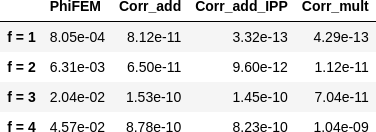
\includegraphics[width=0.8\linewidth]{"corr_ana/tab_errors_phifem_circle.png"}
			\captionof{figure}{Errors $||\cdot||_{L^2,rel}$ obtained with different methods on the Circle with $\phi$-FEM.}
			\label{tab_errors_phifem_circle}
		\end{figure} 
	\end{minipage}
	
	\textbf{Non-homogeneous case :}
	
	We consider here the non-homogeneous problem (i.e. with $\varphi=1$) and seek to test the various correction methods with standard FEM and $\phi$-FEM methods.
	
	\begin{minipage}{0.48\linewidth}
		\begin{figure}[H]
			\centering
			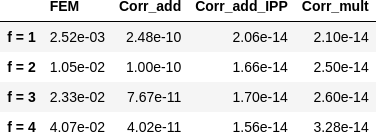
\includegraphics[width=0.8\linewidth]{"corr_ana/tab_errors_fem_circle_nh.png"}
			\captionof{figure}{Errors $||\cdot||_{L^2,rel}$ obtained with different methods on the Circle with standard FEM.}
			\label{tab_errors_fem_circle_nh}
		\end{figure} 
	\end{minipage}
	\begin{minipage}{0.48\linewidth} \qquad 
		\begin{figure}[H]
			\centering
			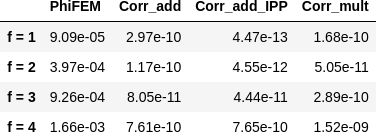
\includegraphics[width=0.8\linewidth]{"corr_ana/tab_errors_phifem_circle_nh.png"}
			\captionof{figure}{Errors $||\cdot||_{L^2,rel}$ obtained with different methods on the Circle with $\phi$-FEM.}
			\label{tab_errors_phifem_circle_nh}
		\end{figure} 
	\end{minipage}
	
	\item \textbf{Results on the Square :}
	
	We consider here the Square problem with the solution defined in Section \ref{Corr.pb.square.1}.
	
	\textbf{Homogeneous case :}
	
	We consider here the homogeneous problem (i.e. with $\varphi=0$) and seek to test the various correction methods with standard FEM and $\phi$-FEM methods.
	
	\begin{minipage}{0.48\linewidth}
		\begin{figure}[H]
			\centering
			\includegraphics[width=0.8\linewidth]{"corr_ana/tab_errors_fem_square.png"}
			\captionof{figure}{Errors $||\cdot||_{L^2,rel}$ obtained with different methods on the Square with standard FEM.}
			\label{tab_errors_fem_square}
		\end{figure} 
	\end{minipage}
	\begin{minipage}{0.48\linewidth} \qquad 
		\begin{figure}[H]
			\centering
			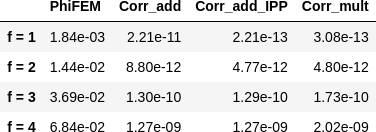
\includegraphics[width=0.8\linewidth]{"corr_ana/tab_errors_phifem_square.png"}
			\captionof{figure}{Errors $||\cdot||_{L^2,rel}$ obtained with different methods on the Square with $\phi$-FEM.}
			\label{tab_errors_phifem_square}
		\end{figure} 
	\end{minipage}
	
	\textbf{Non-homogeneous case :}
	
	We consider here the non-homogeneous problem (i.e. with $\varphi=1$) and seek to test the various correction methods with standard FEM and $\phi$-FEM methods.
	
	\begin{minipage}{0.48\linewidth}
		\begin{figure}[H]
			\centering
			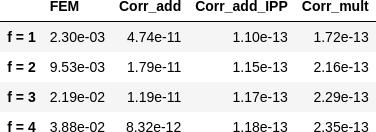
\includegraphics[width=0.8\linewidth]{"corr_ana/tab_errors_fem_square_nh.png"}
			\captionof{figure}{Errors $||\cdot||_{L^2,rel}$ obtained with different methods on the Square with standard FEM.}
			\label{tab_errors_fem_square_nh}
		\end{figure} 
	\end{minipage}
	\begin{minipage}{0.48\linewidth} \qquad 
		\begin{figure}[H]
			\centering
			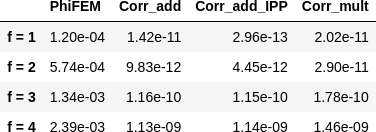
\includegraphics[width=0.8\linewidth]{"corr_ana/tab_errors_phifem_square_nh.png"}
			\captionof{figure}{Errors $||\cdot||_{L^2,rel}$ obtained with different methods on the Square with $\phi$-FEM.}
			\label{tab_errors_phifem_square_nh}
		\end{figure} 
	\end{minipage}
\end{enumerate}

It would therefore seem that the various correction methods work in the different cases considered.

\subsubsection{Correction on disturbed solution} \label{Corr.results.disturbed}
%\graphicspath{{images/corr/corr_pert}}

Now, let's consider a deliberately disturbed solution. The purpose of this step is to check that the correction solvers also work with a solution that is very close to the real solution, but not exact. In this section, we will consider a manually disturbed solution, i.e. the exact solution to which we've added a small, analytically known perturbation.

As explained above, we begin by considering $\tilde{\phi}$ as a manually perturbed solution defined by
\begin{equation*}
	\tilde{\phi}(x,y)=u_{ex}(x,y)+\epsilon P(x,y)
\end{equation*}
where $u_{ex}$ defines the exact solution to the problem, $P$ the perturbation applied to it and $\epsilon$ is a real number that allows the amplitude of the perturbation to be easily increased or decreased. 

\begin{Rem}
	Notice that by taking $\epsilon=0$, we return to the case of correction on an exact solution presented in Section \ref{Corr.results.ana}. 
\end{Rem}

In our case, we will choose to consider $P$ as being of the same form as our exact solution (defined with different parameters), but we could very well consider a completely different perturbation. 

\begin{Rem}
	Note that the shape of the perturbation has a huge influence on the accuracy of the solvers, and that the difficulty lies in the following cases where its expression is not explicitly known (as in the case of $\phi$-FEM in Section \ref{Corr.results.phifem} or FNO in Section \ref{Corr.results.FNO}).
\end{Rem}

In the case of Circle geometry where we consider the problem \ref{Corr.pb.circle.1}, the perturbation will be defined by
\begin{equation*}
	P(x,y)=S_p\times\sin\left(8\pi f_p\left((x-0.5)^2+(y-0.5)^2\right)+\varphi_p\right)
\end{equation*}
where $S_p\in[0,1]$ is the amplitude of the signal, $f_p\in\mathbb{N}$ can be associated with the "frequency" of the signal and $\varphi_p\in[0,1]$ the phase at the origin.

In the case of Square geometry where we consider the problem \ref{Corr.pb.square.1}, the perturbation will be defined by
\begin{equation*}
	P(x,y)=S_p\times\sin\left(2\pi f_px+\varphi_p\right)\times\sin\left(2\pi f_py+\varphi_p\right)
\end{equation*}
where $S_p\in[0,1]$ is the amplitude of the signal, $f_p\in\mathbb{N}$ can be associated with the "frequency" of the signal and $\varphi_p\in[0,1]$ the phase at the origin.

\begin{Rem}
	Note that for the boundary conditions of the solution to be satisfied, i.e. for $\tilde{\phi}=u_{ex}$ on $\Gamma$, it is essential that $P=0$ on $\Gamma$. In the case of both circle and square, we will then take $\varphi_p=0$.
\end{Rem}

Recall the relative errors obtained by standard FEM and $\phi$-FEM on the circle and on the square for frequencies $f\in\{1,2,3,4\}$ for the homogeneous  (Figure \ref{norms}) and non-homogeneous problem  (Figure \ref{norms_nh}).

\begin{minipage}{0.48\linewidth}
	\begin{figure}[H]
		\centering
		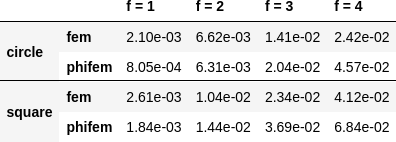
\includegraphics[width=0.8\linewidth]{"corr_pert/diff_eps/norms.png"}
		\captionof{figure}{Table summarizing the errors obtained by standard FEM and $\phi$-FEM on the circle and the square (homogeneous case).}
		\label{norms}
	\end{figure} 
\end{minipage}
\begin{minipage}{0.48\linewidth}
	\begin{figure}[H]
		\centering
		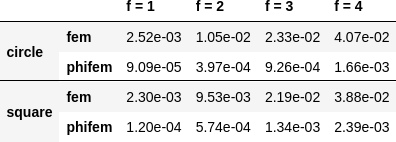
\includegraphics[width=0.8\linewidth]{"corr_pert/diff_eps/norms_nh.png"}
		\captionof{figure}{Table summarizing the errors obtained by standard FEM and $\phi$-FEM on the circle and the square (non-homogeneous case).}
		\label{norms_nh}
	\end{figure} 
\end{minipage}

\paragraph{Results with differents $\epsilon$} \label{Corr.results.disturbed.eps} 

The aim of this section is to test correction by addition (without IPP) and correction by multiplication by varying the amplitude of the perturbation (in other words, by varying $\epsilon$). 

We will try to separate the cases according to the frequencies considered. In other words, for $f,f_p\in\{1,2,3,4\}$, we're interested in the following three cases. The first is the case where the solution frequency is greater than the perturbation frequency ($f>f_p$), i.e. a highly variable solution and a less variable perturbation. The second is where the solution and perturbation frequencies are equal ($f=f_p$), i.e. the solution and perturbation have the same variability. The last category covers cases where the perturbation is "nastier" than the solution, i.e. it has a higher frequency than the solution ($f<f_p$). 

In this section, we'll consider for the circle the solution defined in Section \ref{Corr.pb.circle.1} and for the square the solution defined in Section \ref{Corr.pb.square.1}.

\textbf{Results with standard FEM :}

First we will consider the standard FEM method on the homogeneous case (i.e. with $\varphi=0$) and then on the non-homogeneous case (i.e. with $\varphi=1$).

\begin{enumerate}[label=\textbullet]
	\item \textbf{Results on the homogeneous case :}
	
	First, we consider the correction by adding (without IPP) on the Circle problem (Figure \ref{corr_pert_fem_circle_add}) and on the Square problem (Figure \ref{corr_pert_fem_square_add}).
	
	\begin{minipage}{0.48\linewidth}
		\begin{figure}[H]
			\centering
			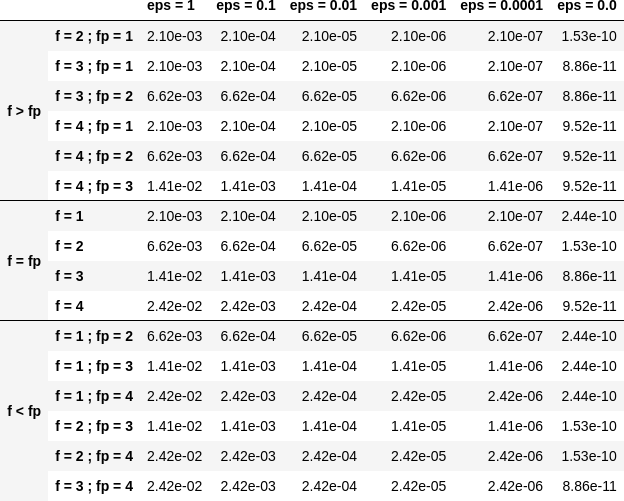
\includegraphics[width=\linewidth]{"corr_pert/diff_eps/fem_circle_add.png"}
			\captionof{figure}{Correction by adding on the Circle with standard FEM in the homogeneous case.}
			\label{corr_pert_fem_circle_add}
		\end{figure} 
	\end{minipage}
	\begin{minipage}{0.48\linewidth}
		\begin{figure}[H]
			\centering
			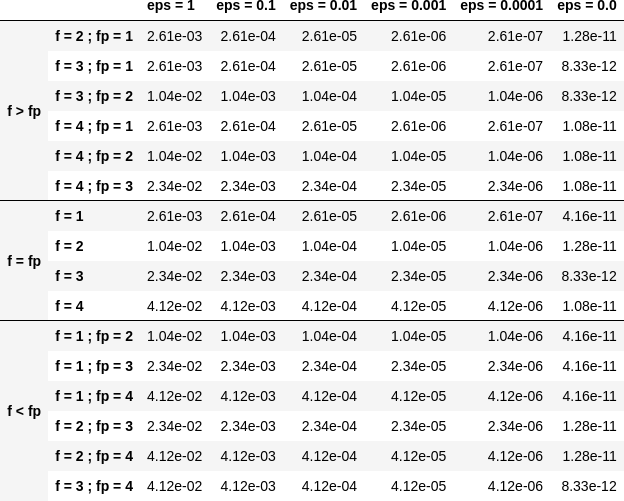
\includegraphics[width=\linewidth]{"corr_pert/diff_eps/fem_square_add.png"}
			\captionof{figure}{Correction by adding on the Square with standard FEM in the homogeneous case.}
			\label{corr_pert_fem_square_add}
		\end{figure} 
	\end{minipage}
	
	Then, we consider the correction by multiplying on the Circle problem (Figure \ref{corr_pert_fem_circle_mult}) and on the Square problem (Figure \ref{corr_pert_fem_square_mult}).
	
	\begin{minipage}{0.48\linewidth}
		\begin{figure}[H]
			\centering
			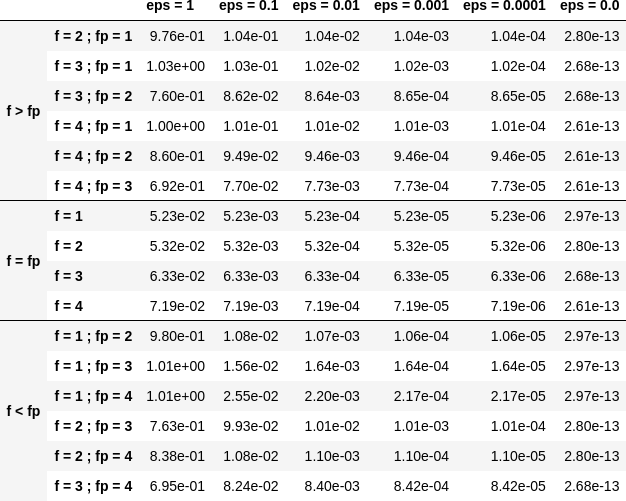
\includegraphics[width=\linewidth]{"corr_pert/diff_eps/fem_circle_mult.png"}
			\captionof{figure}{Correction by multiplying on the Circle with standard FEM in the homogeneous case.}
			\label{corr_pert_fem_circle_mult}
		\end{figure} 
	\end{minipage}
	\begin{minipage}{0.48\linewidth}
		\begin{figure}[H]
			\centering
			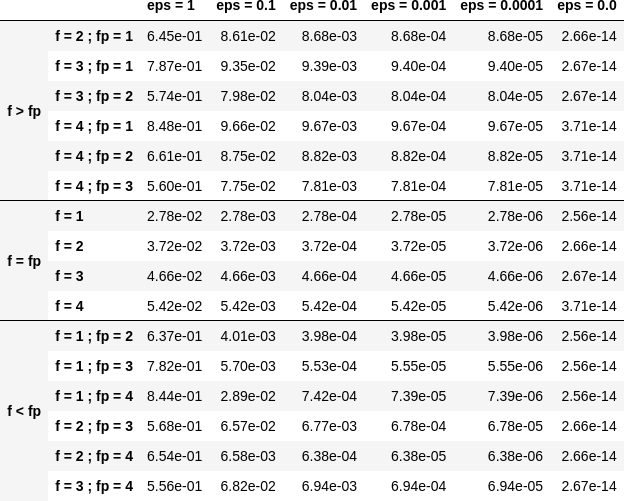
\includegraphics[width=\linewidth]{"corr_pert/diff_eps/fem_square_mult.png"}
			\captionof{figure}{Correction by multiplying on the Square with standard FEM in the homogeneous case.}
			\label{corr_pert_fem_square_mult}
		\end{figure} 
	\end{minipage}
	
	\textbf{\textit{Observation :}} It would therefore seem that, overall, the smaller the perturbation applied (i.e. the smaller the $\epsilon$), the more efficient the addition and multiplication correction solvers are in terms of accuracy. However, we would like to make a few comments on the results obtained:
	\begin{itemize}
		\item First of all, it would appear that, as with the standard FEM and $\phi$-FEM solvers without correction, the more the solution varies (i.e. the larger $f$), the greater the error. This is a fairly intuitive result, since the more the solution varies, the more points are needed to approximate it.
		\item It would also seem that for $\epsilon=1$ (i.e. a large perturbation), this parameter has a greater impact on the multiplicative corrector than on the additive corrector. We explained earlier the benefits of elevating the problem, which could be beneficial here. Results on elevation will be presented in the Section \ref{Corr.results.disturbed.reh}.
		\item In view of the results obtained here, it would also appear that, overall, correction by addition is more effective than correction by multiplication. Moreover, correction by addition has more advantages than correction by multiplication. In particular, if the solution cancels out on the domain, correction by multiplication will require elevating the problem sufficiently so that it no longer cancels out, unlike correction by addition.
	\end{itemize}
	
	\item \textbf{Results on the non-homogeneous case :}
	
	First, we consider the correction by adding (without IPP) on the Circle problem (Figure \ref{corr_pert_fem_circle_add_nh}) and on the Square problem (Figure \ref{corr_pert_fem_square_add_nh}).
	
	\begin{minipage}{0.48\linewidth}
		\begin{figure}[H]
			\centering
			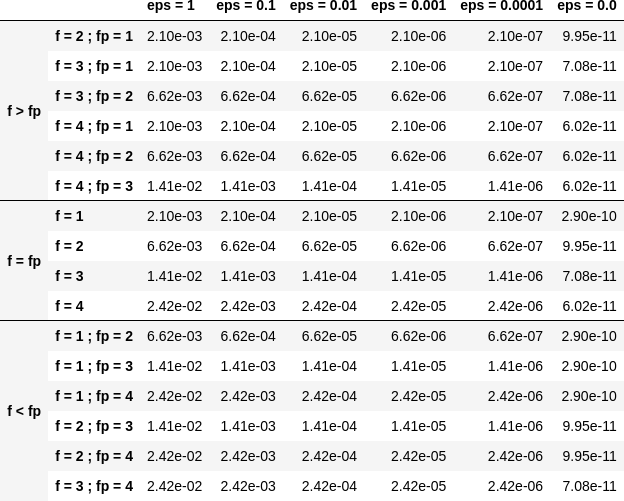
\includegraphics[width=\linewidth]{"corr_pert/diff_eps/fem_circle_add_nh.png"}
			\captionof{figure}{Correction by adding on the Circle with standard FEM in the non-homogeneous case.}
			\label{corr_pert_fem_circle_add_nh}
		\end{figure} 
	\end{minipage}
	\begin{minipage}{0.48\linewidth}
		\begin{figure}[H]
			\centering
			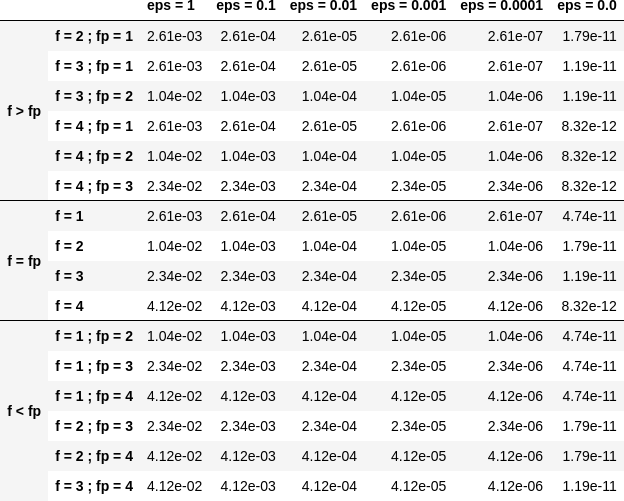
\includegraphics[width=\linewidth]{"corr_pert/diff_eps/fem_square_add_nh.png"}
			\captionof{figure}{Correction by adding on the Square with standard FEM in the non-homogeneous case.}
			\label{corr_pert_fem_square_add_nh}
		\end{figure} 
	\end{minipage}
	
	Then, we consider the correction by multiplying on the Circle problem (Figure \ref{corr_pert_fem_circle_mult_nh}) and on the Square problem (Figure \ref{corr_pert_fem_square_mult_nh}).
	
	\begin{minipage}{0.48\linewidth}
		\begin{figure}[H]
			\centering
			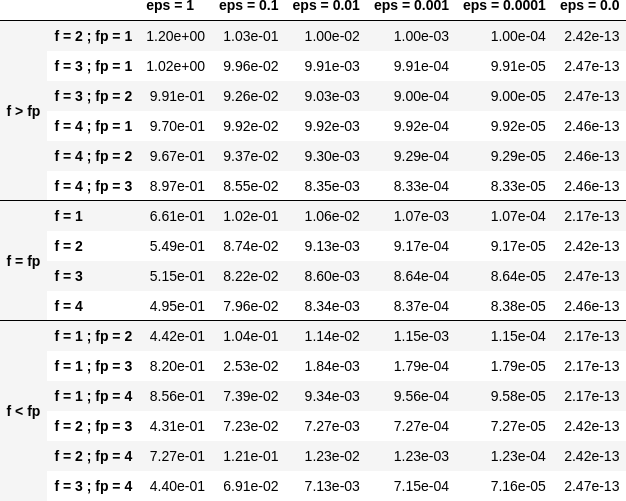
\includegraphics[width=\linewidth]{"corr_pert/diff_eps/fem_circle_mult_nh.png"}
			\captionof{figure}{Correction by multiplying on the Circle with standard FEM in the non-homogeneous case.}
			\label{corr_pert_fem_circle_mult_nh}
		\end{figure} 
	\end{minipage}
	\begin{minipage}{0.48\linewidth}
		\begin{figure}[H]
			\centering
			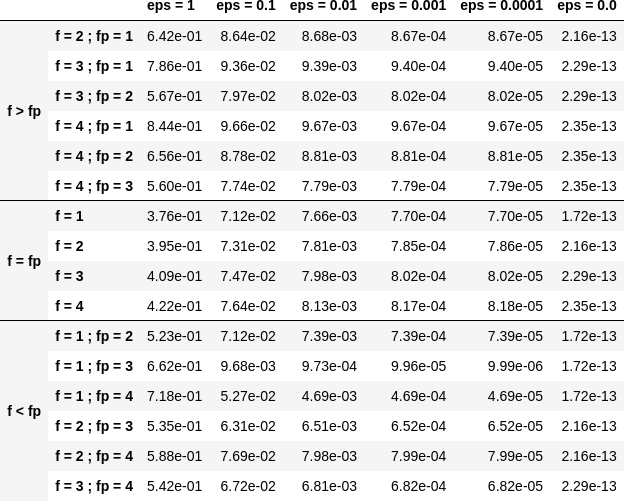
\includegraphics[width=\linewidth]{"corr_pert/diff_eps/fem_square_mult_nh.png"}
			\captionof{figure}{Correction by multiplying on the Square with standard FEM in the non-homogeneous case.}
			\label{corr_pert_fem_square_mult_nh}
		\end{figure} 
	\end{minipage}
	
	\textbf{\textit{Observation :}} In view of the results obtained, it would appear that the conclusions are the same as for the homogeneous case.
\end{enumerate}

\textbf{Results with $\phi$-FEM :}

Then we will consider the $\phi$-FEM method on the homogeneous case (i.e. with $\varphi=0$) and then on the non-homogeneous case (i.e. with $\varphi=1$).

\begin{enumerate}[label=\textbullet]
	\item \textbf{Results on the homogeneous case :}
	
	First, we consider the correction by adding (without IPP) on the Circle problem (Figure \ref{corr_pert_phifem_circle_add}) and on the Square problem (Figure \ref{corr_pert_phifem_square_add}).
	
	\begin{minipage}{0.48\linewidth}
		\begin{figure}[H]
			\centering
			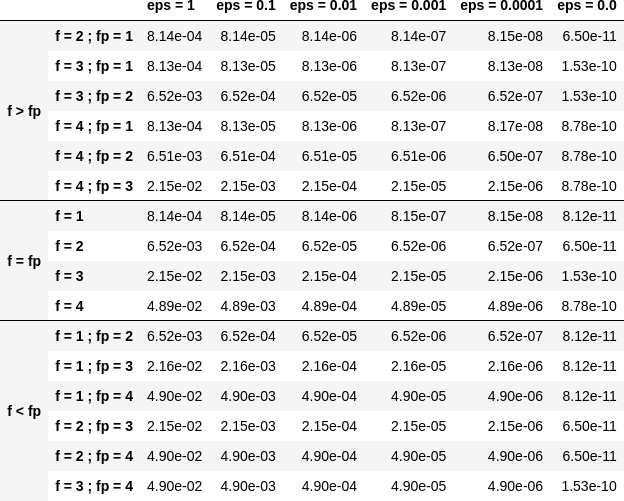
\includegraphics[width=\linewidth]{"corr_pert/diff_eps/phifem_circle_add.png"}
			\captionof{figure}{Correction by adding on the Circle with $\phi$-FEM in the homogeneous case.}
			\label{corr_pert_phifem_circle_add}
		\end{figure} 
	\end{minipage}
	\begin{minipage}{0.48\linewidth}
		\begin{figure}[H]
			\centering
			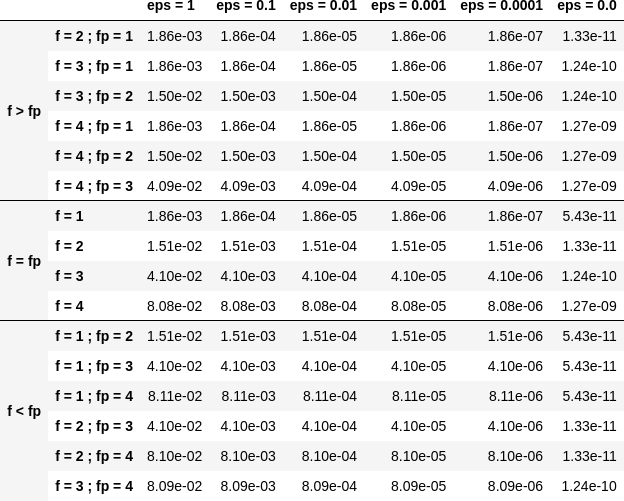
\includegraphics[width=\linewidth]{"corr_pert/diff_eps/phifem_square_add.png"}
			\captionof{figure}{Correction by adding on the Square with $\phi$-FEM in the homogeneous case.}
			\label{corr_pert_phifem_square_add}
		\end{figure} 
	\end{minipage}
	
	Then, we consider the correction by multiplying on the Circle problem (Figure \ref{corr_pert_phifem_circle_mult}) and on the Square problem (Figure \ref{corr_pert_phifem_square_mult}).
	
	\begin{minipage}{0.48\linewidth}
		\begin{figure}[H]
			\centering
			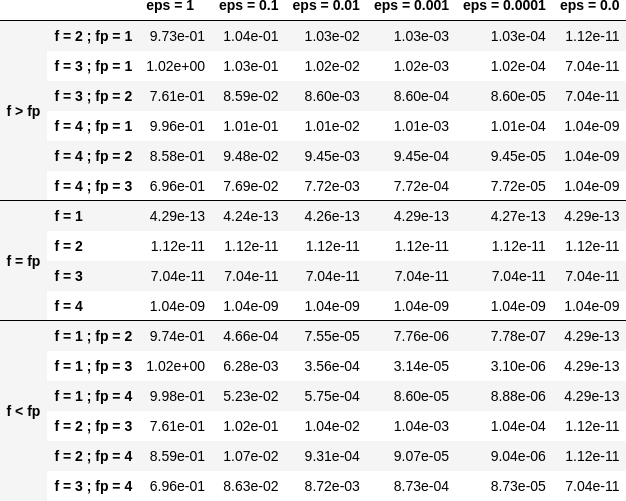
\includegraphics[width=\linewidth]{"corr_pert/diff_eps/phifem_circle_mult.png"}
			\captionof{figure}{Correction by multiplying on the Circle with $\phi$-FEM in the homogeneous case.}
			\label{corr_pert_phifem_circle_mult}
		\end{figure} 
	\end{minipage}
	\begin{minipage}{0.48\linewidth}
		\begin{figure}[H]
			\centering
			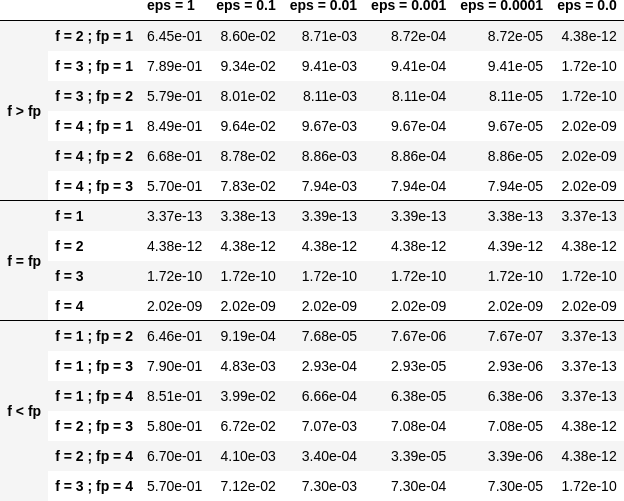
\includegraphics[width=\linewidth]{"corr_pert/diff_eps/phifem_square_mult.png"}
			\captionof{figure}{Correction by multiplying on the Square with $\phi$-FEM in the homogeneous case.}
			\label{corr_pert_phifem_square_mult}
		\end{figure} 
	\end{minipage}
	
	\textbf{\textit{Observation :}} An interesting result can also be observed. Indeed, it seems that in the case where $f=f_p$, the multiplication correction with $\phi$-FEM seems to approach the solution almost perfectly for all $\epsilon$ considered.
	In fact, in the homogeneous case, for $f=f_p$ the perturbation is identical to the solution (i.e. $P=u_{ex}$) and so the solution injected into the correction solvers is of the form
	\begin{equation*}
		\tilde{\phi}=u_{ex}+\epsilon P=(1+\epsilon)u_{ex}
	\end{equation*}
	In the case of correction by multiplication, we have $\tilde{u}=\tilde{\phi}C$. So for $\tilde{u}=u_{ex}$, we must have
	\begin{equation*}
		\tilde{\phi}C=u_{ex} \quad \iff \quad (1+\epsilon)u_{ex}C=u_{ex}
	\end{equation*}
	So if the solution does not cancel out on $\Omega$, we must have
	\begin{equation*}
		C=\frac{1}{1+\epsilon} \quad \text{on } \Omega
	\end{equation*}
	By imposing $C=\frac{1}{1+\epsilon}$ on $\Gamma$ for FEM instead of $C=1$, we should get closer to the $\phi$-FEM results obtained. We can see in Figure \ref{norms_circle_f_eq_fp} and Figure \ref{norms_square_f_eq_fp} that we obtain the expected results for FEM by changing the boundary condition $C=1$ to $C=\frac{1}{1+\epsilon}$.
	
	\begin{minipage}{0.48\linewidth}
		\begin{figure}[H]
			\centering
			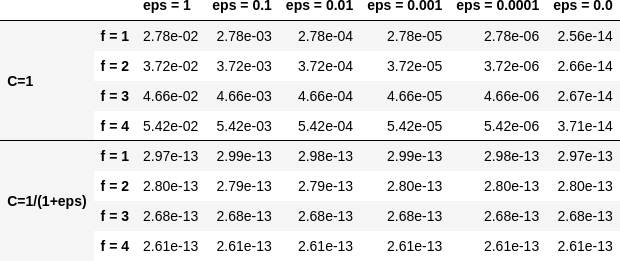
\includegraphics[width=\linewidth]{"corr_pert/diff_eps/norms_circle_f_eq_fp.png"}
			\captionof{figure}{Results by changing FEM boundary conditions on the circle.}
			\label{norms_circle_f_eq_fp}
		\end{figure} 
	\end{minipage}
	\begin{minipage}{0.48\linewidth}
		\begin{figure}[H]
			\centering
			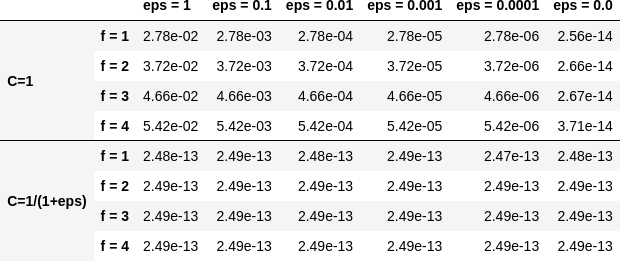
\includegraphics[width=\linewidth]{"corr_pert/diff_eps/norms_square_f_eq_fp.png"}
			\captionof{figure}{Results by changing FEM boundary conditions on the square.}
			\label{norms_square_f_eq_fp}
		\end{figure} 
	\end{minipage}
	\begin{Rem}
		It should be noted, however, that in practice, for example in the case where $\tilde{\phi}$ is a $\phi$-FEM solution or an FNO output, this case is not very realistic. There's no reason to expect the form of the perturbation created by the $\phi$-FEM solver or by the FNO to be exactly identical to the solution under consideration.
	\end{Rem}
	
	\item \textbf{Results on the non-homogeneous case :}
	
	First, we consider the correction by adding (without IPP) on the Circle problem (Figure \ref{corr_pert_phifem_circle_add_nh}) and on the Square problem (Figure \ref{corr_pert_phifem_square_add_nh}).
	
	\begin{minipage}{0.48\linewidth}
		\begin{figure}[H]
			\centering
			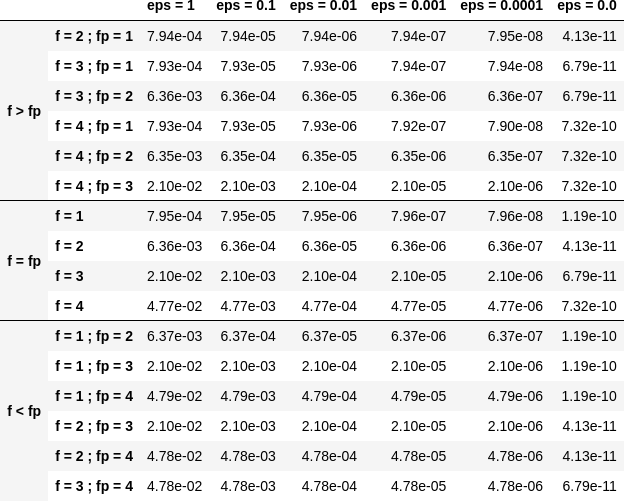
\includegraphics[width=\linewidth]{"corr_pert/diff_eps/phifem_circle_add_nh.png"}
			\captionof{figure}{Correction by adding on the Circle with $\phi$-FEM in the non-homogeneous case.}
			\label{corr_pert_phifem_circle_add_nh}
		\end{figure} 
	\end{minipage}
	\begin{minipage}{0.48\linewidth}
		\begin{figure}[H]
			\centering
			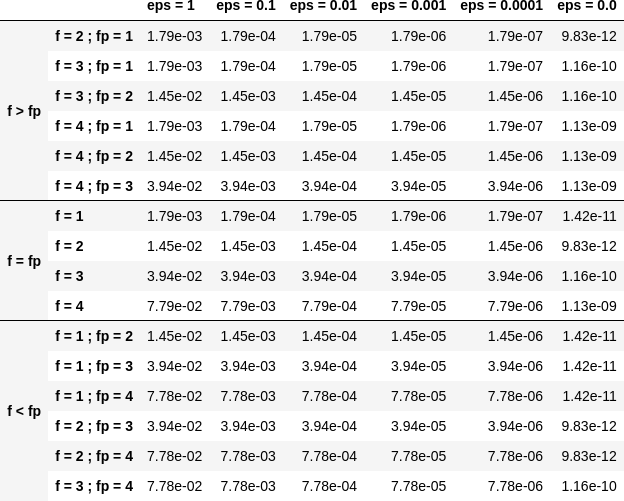
\includegraphics[width=\linewidth]{"corr_pert/diff_eps/phifem_square_add_nh.png"}
			\captionof{figure}{Correction by adding on the Square with $\phi$-FEM in the non-homogeneous case.}
			\label{corr_pert_phifem_square_add_nh}
		\end{figure} 
	\end{minipage}
	
	Then, we consider the correction by multiplying on the Circle problem (Figure \ref{corr_pert_phifem_circle_mult_nh}) and on the Square problem (Figure \ref{corr_pert_phifem_square_mult_nh}).
	
	\begin{minipage}{0.48\linewidth}
		\begin{figure}[H]
			\centering
			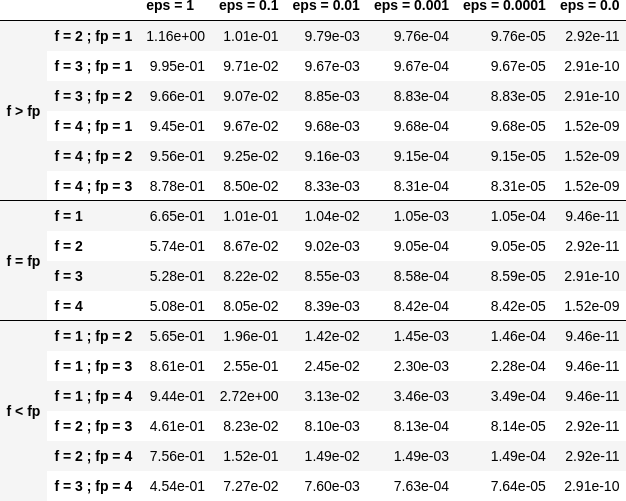
\includegraphics[width=\linewidth]{"corr_pert/diff_eps/phifem_circle_mult_nh.png"}
			\captionof{figure}{Correction by multiplying on the Circle with $\phi$-FEM in the non-homogeneous case.}
			\label{corr_pert_phifem_circle_mult_nh}
		\end{figure} 
	\end{minipage}
	\begin{minipage}{0.48\linewidth}
		\begin{figure}[H]
			\centering
			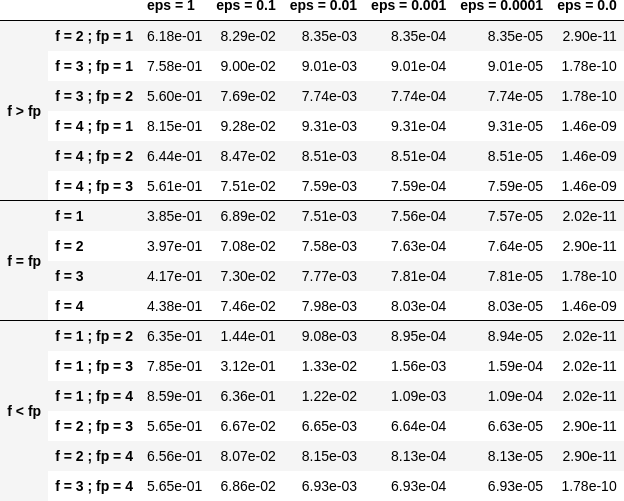
\includegraphics[width=\linewidth]{"corr_pert/diff_eps/phifem_square_mult_nh.png"}
			\captionof{figure}{Correction by multiplying on the Square with $\phi$-FEM in the non-homogeneous case.}
			\label{corr_pert_phifem_square_mult_nh}
		\end{figure} 
	\end{minipage}
	
	\textbf{\textit{Observation :}} In view of the results obtained, it would appear that the conclusions are the same as for the homogeneous case. Except for the case where $f=f_p$, because in the case where the solution is non-homogeneous (i.e. $u_{ex}=g$ on $\Gamma$), the perturbation $P$ is no longer equal to the solution $u_{ex}$ because $P=0$ on $\Gamma$.
\end{enumerate}


\paragraph{Results on the elevated problem} \label{Corr.results.disturbed.reh} 

In this section, we aim to show numerically the interest of elevating the problem. To do this, we'll consider the case of the circle with the solution defined in Section \ref{Corr.pb.circle.1} and the case of the square with the solution defined in Section \ref{Corr.pb.square.1}. We'll choose the homogeneous case (i.e. with $\varphi=0$) with $S=0.5$ and set $\epsilon=10^{-3}$.

\textbf{Results with FEM :}

	Here, we consider some of the cases considered above, in order to test that elevating the solution is useful, a method presented in Section \ref{Corr.method.mult_reh}. We'll test this method on the circle and on the square for selected frequencies and by varying $m$.

	\begin{minipage}{0.48\linewidth}
		\begin{figure}[H]
			\centering
			\includegraphics[width=\linewidth]{"corr_pert/rehaussement/tab_errors_fem_circle.png"}
			\captionof{figure}{Correction by multiplying on the elevated problem on the Circle with FEM.}
			\label{corr_pert_fem_circle_reh}
		\end{figure} 
	\end{minipage}
	\begin{minipage}{0.48\linewidth}
		\begin{figure}[H]
			\centering
			\includegraphics[width=\linewidth]{"corr_pert/rehaussement/tab_errors_fem_square.png"}
			\captionof{figure}{Correction by multiplying on the elevated problem on the Square with FEM.}
			\label{corr_pert_fem_square_reh}
		\end{figure} 
	\end{minipage}
	
	\begin{minipage}{0.48\linewidth}
		\begin{figure}[H]
			\centering
			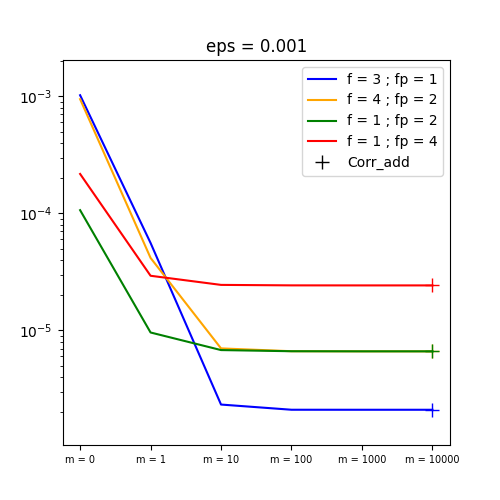
\includegraphics[width=0.8\linewidth]{"corr_pert/rehaussement/fig_fem_circle.png"}
			\captionof{figure}{Representation of the results on the Circle with FEM.}
			\label{corr_pert_fem_circle_reh_fig}
		\end{figure} 
	\end{minipage}
	\begin{minipage}{0.48\linewidth}
		\begin{figure}[H]
			\centering
			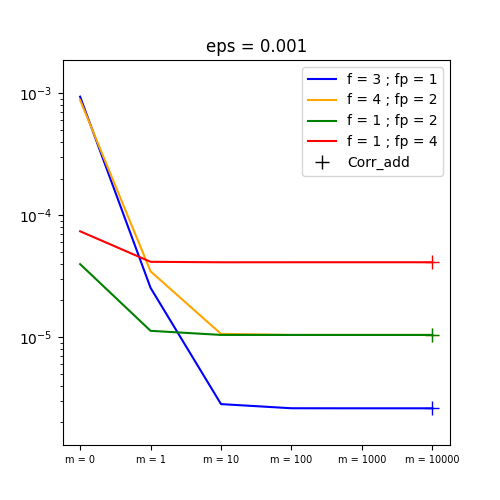
\includegraphics[width=0.8\linewidth]{"corr_pert/rehaussement/fig_fem_square.png"}
			\captionof{figure}{Representation of the results on the Square with FEM.}
			\label{corr_pert_fem_square_reh_fig}
		\end{figure} 
	\end{minipage}
	 
	\textbf{Observation :} The numerical results obtained on the circle in Figure \ref{corr_pert_fem_circle_reh} and on the square \ref{corr_pert_fem_square_reh}, seem to show that the higher we raise the problem, the better the error. Furthermore, as explained in \modif{add section}, we can see that by increasing $m$, the error converges to the error obtained with the correction by adding and therefore the solution itself converges to the solution obtained with the correction by adding. 


\subsubsection{Correction on $\phi$-FEM solution} \label{Corr.results.phifem}

\modif{Then we'll look at correcting a disturbed solution for which we don't know the form of the perturbation. A $\phi$-FEM solution can be considered for injection into correction solvers.}

\subsubsection{Correction with FNO} \label{Corr.results.FNO}

\subsubsection{Correction with other networks} \label{Corr.results.neural_net}

\paragraph{Multiperceptron} \label{Corr.results.neural_net.multiperceptron}

\paragraph{PINNs} \label{Corr.results.neural_net.PINNs}